\documentclass[10pt,a4paper]{report}
\usepackage[latin1]{inputenc}
%\usepackage[utf8x]{inputenc}
\usepackage[english]{babel}
\usepackage{amsmath}
\usepackage{amsfonts}
\usepackage{amssymb}
\usepackage{graphicx}
\usepackage{verbatim}
\usepackage[left=1.5cm,right=1.5cm,top=2.5cm,bottom=2.5cm]{geometry}

\pagenumbering{gobble}

\DeclareMathOperator{\ind}{\perp \!\!\! \perp}



% Le document est sur 6 pages organisées comme ci-dessous :
% 1 3 5
% 2 4 6

% Tu as acc�s � une imprimante (facilement) ?
\begin{document}

\begin{center}
\resizebox{\linewidth}{!}{\itshape \textbf{Generalization and}}
\end{center}
\vspace{80pt}

\begin{center}
\Huge{\textit{Introduction}}
\end{center}
\vspace{20pt}

\Large{
	
	Hidden Markov Models (HMMs) are widely used for probabilistic models of time series data. Here we used a generalization of HMMs called factorial hidden Markov model, in which a state $S_t$ corresponding to an hidden variable is now represented by a collection of states $S_t = \left(S_t^{(1)},\dots,S_t^{(M)}\right)$ each of which can take $K^{(m)}$ values (figure (a)). Here we consider the case where $K = K^{(m)}$ for all $m$. Furthermore, we assume that $\{(S_t^{(m)})_{t=0}^T\}_{m=0}^M$ are independent Markov chains and that the observation $y_t$ are Gaussian random vector whose mean is a linear function of the hidden variables and have the same covariance matrix $C$.
	\newline
	\newline
	
	}

\begin{figure}[h]
	\centering
	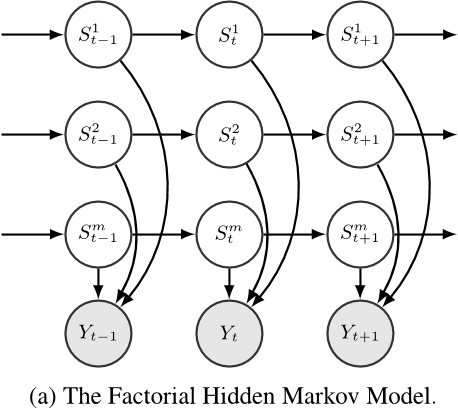
\includegraphics[width=0.6\textwidth]{fHMM.png}
	%\centerline{Factorial Hidden Markov Model}
	\label{fig:a}
\end{figure}


\newpage
\begin{center}
\Huge{\textit{Inference and learning}}
\end{center}
\vspace{20pt}

\Large{

Here we want to learn the parameters of a factorial HMM for a given structure. For that we use the EM algorithm to estimate them. While the M step is simple and tractable, the E step is computationally more difficult. We have four options:

\begin{itemize}
	\item[-]Exact inference: it is computationally intractable for a big model.
	\item[-]Inference using Gibbs sampling.
	\item[-]Completely factorized variational inference: we approximate the posterior distribution by a tractable distribution and we make the assumption that all the hidden variables are independent.
	\item[-]Structured variational inference: same as above but we take into account the structure of the hidden variables (figure(b)).
\end{itemize}

}

\begin{figure}[h]
	\centering
	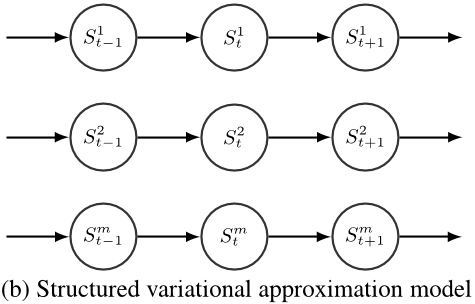
\includegraphics[width=0.6\textwidth]{sva.png}
	%\centerline{Factorial Hidden Markov Model}
	\label{fig:b}
\end{figure}








\newpage
\begin{center}
\resizebox{\linewidth}{!}{\itshape \textbf{acceleration of HMMs}}
\end{center}
\vspace{5pt}
\begin{center}
	\LARGE{Matthieu Jedor \& Alban Pierre}
	\vspace{15pt}
	
	\Large{Keywords: Hidden Markov models, time series, EM algorithm, graphical models, Bayesian networks, mean field
theory}
\end{center}
\vspace{30pt}
\begin{center}
\Huge{\textit{Experiments on synthetic data}}
\end{center}
\vspace{20pt}
\Large{
	We generate synthetic datasets using a factorial hidden Markov model and then we tried to learn the parameters with our 4 algorithms. Figure 1 shows the log-likelihood accross iterations and figure (d) shows the results in terms of centers found.
	
}

TODO add log-likelihood plots and time of computation, and the protocol of experimentations

\newpage


\begin{figure}[h]
	\centering
	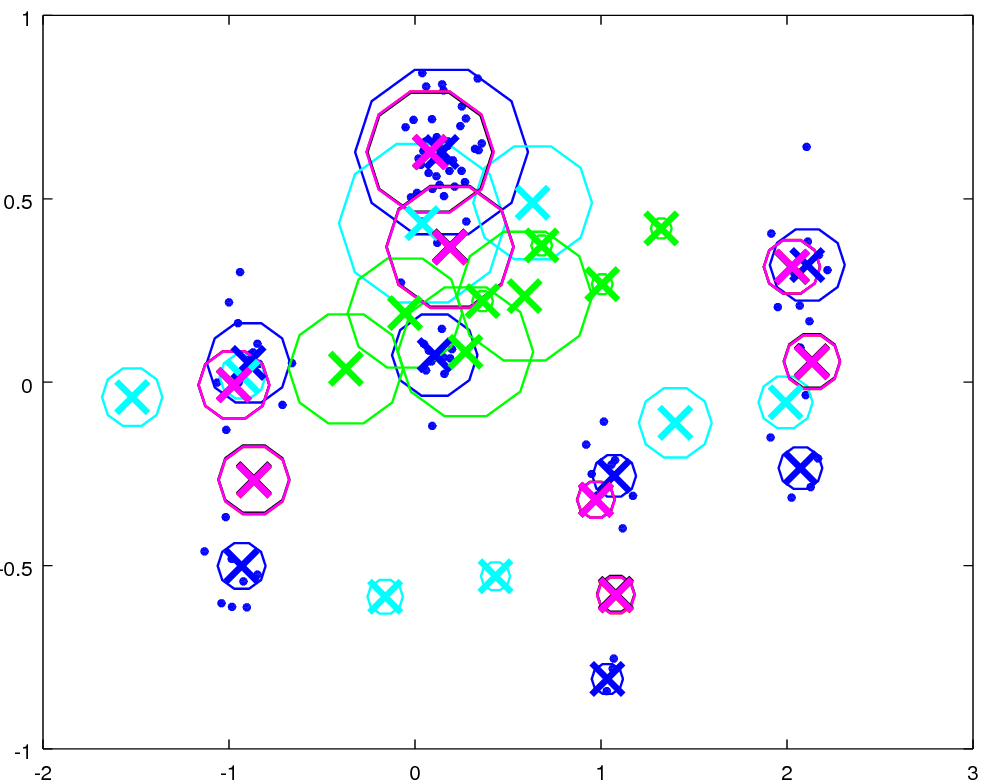
\includegraphics[width=0.8\textwidth]{fig11.png}
	\centerline{\Large{(d) Centers on synthetic data}}
	\label{fig:c}
\end{figure}
\begin{center}
	Cross = centers, Circles = probabilities of each center
	
	Blue = True parameters
	
	Light Blue = Kmeans Initialization
	
	Violet = FHMM, CFVA, SVA (they found the same result)
	
	Green = Gibbs sampling
	
\end{center}
\vspace{30pt}

The initialization of parameters is very important. With a random initialization, we achieved poor results as half centers found by our algorithms or less matched the whole data and the other half ended in the middle of nowhere. So we used a recursive K-means initialization, which works as follow : (with $W$ defining the centers : $\mu_t = W*S_t$ ; and $P$ the transition matrix)

\begin{verbatim}
For m = 1 to M
     k = kmeans with K centers
     Superpose each cluster found
     The m-th set of K columns of W = k
     The m-th set of K lines of P = probability of clusters k
endFor
\end{verbatim}






\clearpage
\begin{center}
\resizebox{\linewidth}{!}{\itshape \textbf{using factorial HMMs}}
\end{center}
\vspace{80pt}
\begin{center}
\Huge{\textit{Experiments on real data}}
\end{center}
\vspace{20pt}

We applied the structural variational approximation on real data. First we choose the dataset "Activity Recognition from Single Chest-Mounted Accelerometer Data Set" from UCI Repository, which records the acceleration of persons during different activities such as walking, going up/down stairs or working at computer. We tried to learn parameters of each of theses activities, and then for a new activity we compute the log-likelihood of each set of parameters, and the set of parameters that gave the biggest log-likelihood would be the recognized activity. In practice the data is not separated in several gaussians (figure (e)) so it performs very bad at recognizing activities.

\begin{figure}[h]
	\centering
	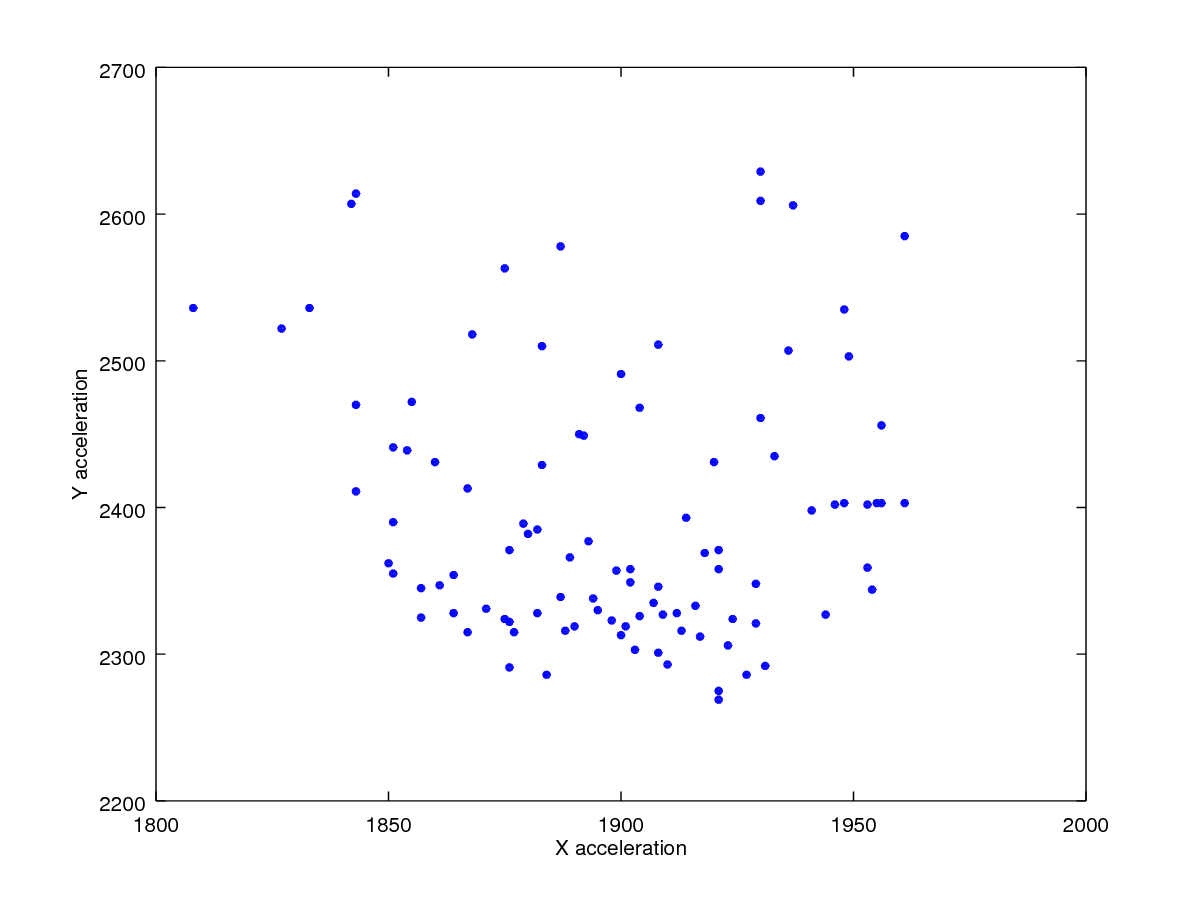
\includegraphics[width=0.7\textwidth]{standing.png}
	\centerline{\Large{Example of data from the Single Chest-Mounted Accelerometer Data Set}}
	\label{fig:e}
\end{figure}

\newpage
Then we tried another dataset : CalIt2 Building People Counts Data Set, which counts the number of persons that come in and out of a building.





\iffalse

\begin{figure}[h]
	\centering
	\includegraphics[width=1.0\textwidth]{P2.png}
	\centerline{Paramètres utilisés pour calculer les probabilités des états cachés}
	\label{fig:d}
\end{figure}


\begin{tabular}{lcc}
	& Entrainement & Test \\
	EM mixture de gaussiennes & -2371 & -2453 \\
	EM chaine de Markov cachée & -1899 & -1957 \\
\end{tabular}
\newline

\fi

\end{document}
